%
% SOLVEURS INTEGRES
%
\subsection{Solveurs intégrés}


%
% SOLVEURS EXTERNES
%
\subsection{Intégration avec des solveurs externes}

\noindent La plupart des solveurs SAT et QBF acceptent le format standard~\href{http://www.satcompetition.org/2009/format-benchmarks2009.html}{DIMACS} (resp.
QDIMACS) comme langage d'entrée. Il suffit de donner la sortie DIMACS de \touist directement à un solveur et d'utiliser la table de correspondance (voir Section~\ref{mapping-table}).
Mais il est également possible d'utiliser \touist pour effectuer à la fois l'appel d'un solveur externe et la traduction inverse du modèle DIMACS retourné par ce dernier vers les noms de variables propositionnelles en utilisant l'argument \mdcode{--solver}:%mdk
\begin{footnotesize}
\begin{mdpre}%mdk
\noindent\preindent{4}touist~{}[--sat\textbar{}--qbf]~--solver="\textless{}cmd-and-arguments\textgreater{}"~{}[--verbose]%mdk
\end{mdpre}
\end{footnotesize}
\noindent A des fins de débogage, il est possible d'ajouter \mdcode{--verbose} pour afficher les entrée et sorties stdin/stdout/stderr.
Le code de sortie de \touist sera alors le même qu'en utilisant \mdcode{--solve}.

Les solveurs externes doivent utiliser les conventions Minisat + (Q)DIMACS suivantes :
\begin{itemize}
    \item accepter DIMACS ou QDIMACS sur l'entrée standard (stdin) ;
    \item afficher un modèle (ou un modèle partiel) au format DIMACS sur la sortie standard (stdout) ; le modèle peut éventuellement être étendu sur plusieurs lignes, chacune commençant par \mdcode{v}, \mdcode{V} ou rien (pour la compatibilité avec Minisat), et chaque ligne peut de manière optionnelle se terminer par 0.
%\end{itemize}%mdk
\begin{mdpre}%mdk
\noindent\preindent{2}v~-1~2~-3~4~0\\
\preindent{2}v~5~-6~0%mdk
\end{mdpre}
%\begin{itemize}[noitemsep,topsep=\mdcompacttopsep]%mdk

\item retourner 10 (comme code d'erreur) sur le problème est SAT, 20 s'il est UNSAT.%mdk
%mdk
\end{itemize}%mdk

\noindent Les solveurs SAT que nous avons testés (\mdcode{brew} est disponible pour~\href{http://linuxbrew.sh}{linux} et~\href{https://brew.sh}{mac}):%mdk

\begin{itemize}%mdk

\item{}
\href{http://minisat.se}{minisat}%mdk
\begin{footnotesize}
\begin{mdpre}%mdk
\noindent brew~install~minisat\\
touist~test/sat/sudoku.touist~--solver="minisat~/dev/stdin~/dev/stdout"%mdk
\end{mdpre}%mdk
\end{footnotesize}

\item{}
\href{http://fmv.jku.at/picosat}{picosat} (2015, version 965, SAT Race'15)%mdk
\begin{footnotesize}
\begin{mdpre}%mdk
\noindent brew~install~touist/touist/picosat\\
touist~test/sat/sudoku.touist~--solver="picosat~--partial"%mdk
\end{mdpre}%mdk
\end{footnotesize}

\item{}
\href{https://www.labri.fr/perso/lsimon/glucose}{glucose} (2016, version 4.1, syrup est la version parallèle)%mdk
\begin{footnotesize}
\begin{mdpre}%mdk
\noindent brew~install~touist/touist/glucose\\
touist~test/sat/sudoku.touist~--solver="glucose~-model"\\
touist~test/sat/sudoku.touist~--solver="glucose-syrup~-model"%mdk
\end{mdpre}%mdk
\end{footnotesize}%mdk
\end{itemize}%mdk

\noindent Les solveurs QBF que nous avons testés:%mdk

\begin{itemize}%mdk

\item{}
\href{https://www.react.uni-saarland.de/tools/caqe/index.html}{caqe} (2017-07-19, CAQE qbfeval 2017, version binaire sans certification).
Download the version \emph{CAQE qbfeval 2017 (2017-07-19) binary release without certification}
which will give you \mdcode{caqe-mac}:%mdk
\begin{footnotesize}
\begin{mdpre}%mdk
\noindent touist~test/qbf/allumettes2.touist~--qbf~--solver="./caqe-mac~--partial-assignments"%mdk
\end{mdpre}
\end{footnotesize}

They also have a Homebrew tap repository but this version does not contain
the needed \mdcode{--partial-assignments}.%mdk%mdk

\item{}
\href{https://github.com/perebor/qute}{qute} (2017-02-27, fork maelvalais/qute, minisat-based)%mdk
\begin{mdpre}%mdk
\noindent brew~install~touist/touist/qute\\
touist~test/qbf/allumettes2.touist~--qbf~--solver="qute~--partial-certificate"%mdk
\end{mdpre}%mdk

\item{}
\href{http://lonsing.github.io/depqbf/}{depqbf} (2017-08-02, DepQBF 6.03, Minisat-based QCDCL)%mdk
\begin{mdpre}%mdk
\noindent brew~install~depqbf\\
touist~test/qbf/allumettes2.touist~--qbf~--solver="depqbf~--qdo~--no-dynamic-nenofex"%mdk
\end{mdpre}%mdk

\item{}
\href{http://fmv.jku.at/quantor/}{quantor} (2014-10-26, Quantor 3.2). It is not necessary to use this
solver externally as it is included with \mdcode{touist} (see Section~\ref{usage-qbf-solver}).%mdk
\begin{mdpre}%mdk
\noindent brew~install~touist/touist/quantor\\
touist~test/qbf/allumettes2.touist~--qbf~--solver="quantor"%mdk
\end{mdpre}%mdk

\item{}
\href{http://sat.inesc-id.pt/~mikolas/sw/areqs/}{rareqs} (2012, v1.1, CEGAR)%mdk
\begin{mdpre}%mdk
\noindent brew~install~touist/touist/rareqs\\
touist~test/qbf/allumettes2.touist~--qbf~--solver="rareqs"%mdk
\end{mdpre}%mdk
%mdk
\end{itemize}%mdk


%
% AUTRES SORTIES
%
\subsection{Autres sorties (\LaTeX...)}


%%%%
\fred{SECTION DU MANUEL A UTILISER}


\paragraph*{3.1.\hspace*{0.5em}Installation}\label{sec-installation}%mdk%mdk

\noindent The main tool that parses and solves the {\scshape TouIST} programs is written in
Ocaml. It is easily installable (as long as you have installed \mdcode{ocaml}
and \mdcode{opam}) with the command%mdk
\begin{mdpre}%mdk
\noindent\preindent{4}opam~install~touist%mdk
\end{mdpre}
\noindent\textbf{Note}.
By default, \mdcode{touist} only comes with a SAT solver. Problems written in
{\scshape TouIST} using the Satisfiability Modulo Theory (SMT) or Quantified
Boolean Formulas (QBF) grammars can also be used (see Sections~\ref{usage-smt} and
\ref{usage-qbf}).%mdk%mdk

\noindent\mdinline{vertical-align=middle}{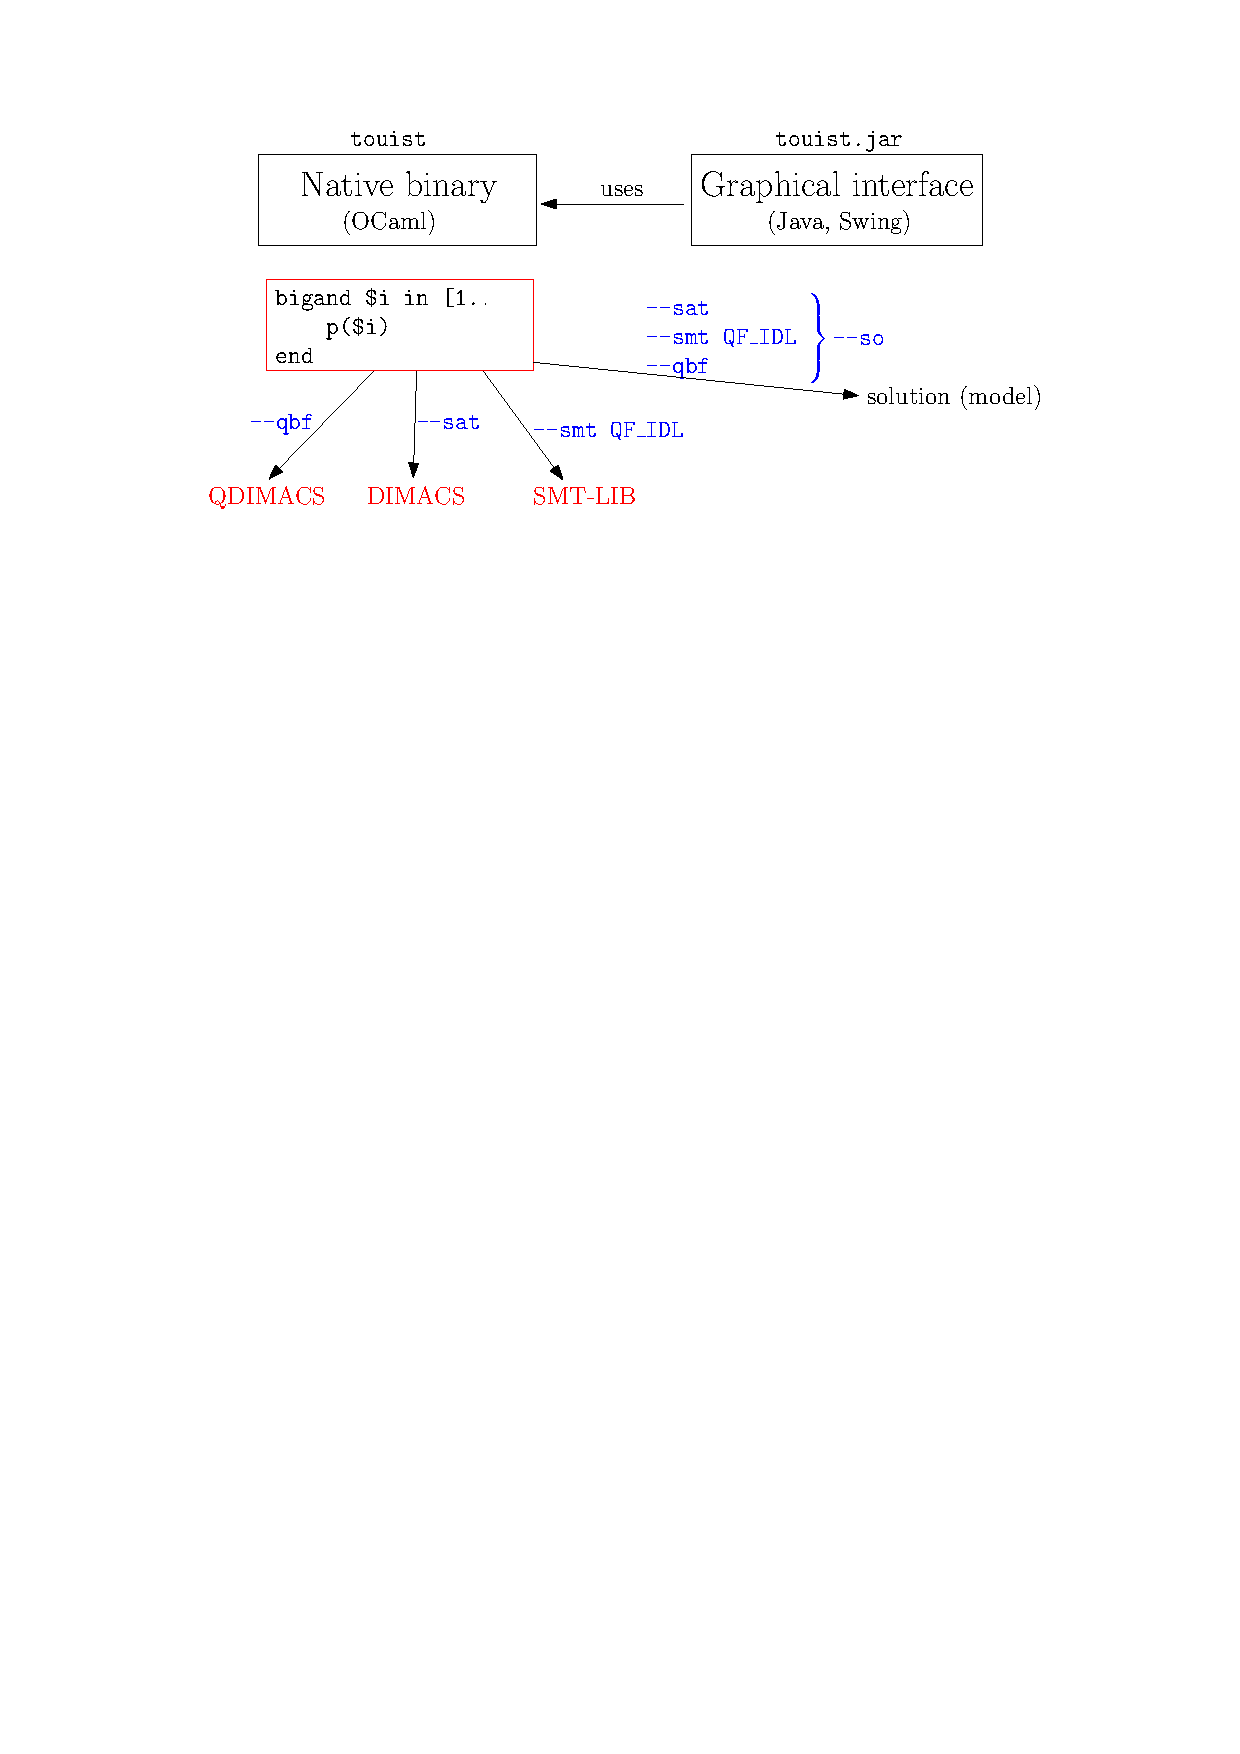
\includegraphics[keepaspectratio=true,width=\dimwidth{1.00}]{figures/architecture}{}}%mdk


\paragraph*{3.2.\hspace*{0.5em}Usage}\label{cli}%mdk%mdk

\noindent Any \mdcode{touist} command is of the form:%mdk
\begin{mdpre}%mdk
\noindent\preindent{4}touist~{}[-o~OUTPUT]~(INPUT~\textbar{}~-)~{}[options...]%mdk
\end{mdpre}\noindent The flags can be given in any order. You can use the standard input
(\mdcode{stdin}) instead of using an input file by setting the \mdcode{-} argument.
With no \mdcode{-o} flag, \mdcode{touist} will output to the standard output (\mdcode{stdout}).

The man page of \mdcode{touist} is available through \mdcode{man~touist} or \mdcode{touist~--help}.
It contains almost everything you need to know its features and arguments.%mdk

%sub
\paragraph*{3.2.1.\hspace*{0.5em}Exit status}\label{sec-exit-status}%mdk%mdk
\begin{mdtabular}{3}{\dimeval{(\linewidth)/3}}{1ex}%mdk
\begin{tabular}{cll}\midrule
{\bfseries Code}&\multicolumn{1}{c}{{\bfseries Label}}&\multicolumn{1}{c}{{\bfseries Description}}\\

\midrule
0&\mdcode{OK~~~~~~~~~~~~~}&with \textendash{}solve or \textendash{}solver, means SAT\\
8&\mdcode{UNSAT~~~~~~~~~~}&with \textendash{}solve or \textendash{}solver, means UNSAT\\
50&\mdcode{TRANSL\_ERROR~~~~~~}&any error of syntax, type or during the translation\\
100&\mdcode{SOLVER\_ERROR}&any solver error (memory overflow, wrong something\dots{})\\
124&\mdcode{CLI\_ERROR~~}&something wrong with the command-line arguments\\
125&\mdcode{BUG~~~}&the solver did not find any model\\
9&\mdcode{SOLVER\_UNKNOWN~}&\\
\midrule
\end{tabular}\end{mdtabular}

\noindent Note that the \mdcode{UNSAT} is not really an error, but we choose to return a
non-zero exit status anyway.%mdk

%sub
\paragraph*{3.2.2.\hspace*{0.5em}Usage for propositional logic (SAT mode)}\label{usage-sat}%mdk%mdk

\noindent The language accepted for propositional logic is described in
\ref{sec-propositional-logic-formulas}. This mode is enabled by
default, but can be optionally expressed using the \mdcode{--sat} flag.%mdk

\subsubsection{Mapping table for DIMACS output}\label{mapping-table}%mdk%mdk

\noindent With no other argument, \mdcode{touist} will simply translate the {\scshape TouIST} code to
the~\href{http://www.satcompetition.org/2009/format-benchmarks2009.html}{DIMACS} format and then output the mapping table (that maps
each proposition to an integer \textgreater{} 0) in DIMACS comments before the prelude
line (i.e., \mdcode{p~cnf~x~y}; comments must be before the prelude line in the
\href{http://www.satcompetition.org/2009/format-benchmarks2009.html}{DIMACS specification}). For example, if you run:%mdk
\begin{mdpre}%mdk
\noindent\preindent{4}echo~'rain~=\textgreater{}~wet\_road~rain~not~wet\_road'~\textbar{}~touist~-%mdk
\end{mdpre}\noindent you will get the output:
\begin{mdpre}%mdk
\noindent\preindent{4}c~wet\_road~1~~~~~~~~~~\textless{}-~mapping~between~DIMACS~integers~and~propositions\\
\preindent{4}c~rain~2\\
\preindent{4}p~cnf~2~3~~~~~~~~~~~~~\textless{}-~prelude~of~the~DIMACS~file\\
\preindent{4}1~-2~0\\
\preindent{4}2~0\\
\preindent{4}-1~0%mdk
\end{mdpre}\noindent You can redirect this mapping table using the \mdcode{--table~\textless{}filename\textgreater{}} flag.

\subsubsection{SAT solver}\label{usage-sat-solver}%mdk%mdk

\noindent By default, \mdcode{touist} embeds~\href{http://minisat.se}{Minisat}
(see~[\cite{sorensson02minisatv1_13}{6}]), a SAT solver written in C++ at the
Chalmers University of Technology, Sweden. It is distributed under the
MIT license. To be able to embed it into OCaml, we use the
binding~\href{https://github.com/c-cube/ocaml-minisat}{ocaml-minisat} which relies on a C version of Minisat
(Minisat-C-1.14.1) for portability concerns.%mdk

\textbf{\mdcode{--solve}} asks \mdcode{touist} to solve the SAT problem. By default, the first
model is displayed; you can ask for more models using the \mdcode{--limit~N}
option. The models are separated by lines beginning with \mdcode{====} and for
one model, each line contains a valuation followed by the corresponding
proposition. For example:%mdk
\begin{mdpre}%mdk
\noindent\preindent{4}echo~a~and~b~\textbar{}~touist~-~--solve%mdk
\end{mdpre}\noindent will return a single model (and in this case, there is only one single model):
\begin{mdpre}%mdk
\noindent\preindent{4}1~a\\
\preindent{4}1~b%mdk
\end{mdpre}\noindent Each line corresponds to a valuation, and each valuation should be read
\mdcode{value~proposition}. In the example, $a$ takes the value 1 (true).
With this format, you can easily filter the results. For example,
the following command will only show the propositions that are \mdcode{{\mdcolor{navy}true}}:
\begin{mdpre}%mdk
\noindent\preindent{4}echo~a~and~b~\textbar{}~touist~-~--solve~\textbar{}~grep~\textasciicircum{}1%mdk
\end{mdpre}\noindent**\mdcode{--solve~--interactive} allows the user to display the models one after
the other. Press enter or any other key to continue and \mdcode{q} or \mdcode{n} to stop.

\textbf{\mdcode{--solve~--limit~N}} allows to display multiple models. With this option,
the models are separated by lines beginning with \mdcode{====} and for one model,
each line contains a valuation followed by the corresponding proposition.
For example, with \mdcode{--limit~0} which displays an unlimited number of models:%mdk
\begin{mdpre}%mdk
\noindent\preindent{4}echo~a~or~b~\textbar{}~touist~-~--solve~--limit~0%mdk
\end{mdpre}\noindent will display
\begin{mdpre}%mdk
\noindent\preindent{4}====~model~0\\
\preindent{4}1~a\\
\preindent{4}0~b\\
\preindent{4}====~model~1\\
\preindent{4}0~a\\
\preindent{4}1~b\\
\preindent{4}====~model~2\\
\preindent{4}1~a\\
\preindent{4}1~b\\
\preindent{4}====~found~3~models,~limit~is~0~(--limit~N~for~more~models)%mdk
\end{mdpre}\noindent Note that the model counter begins at 0.

\textbf{\mdcode{--solve~--count}} tries to return the count of models instead of
returning the models. This option will only work for small problems: the
number of models explodes when the number of propositions is big.%mdk

%sub
\paragraph*{3.2.3.\hspace*{0.5em}Other general options}\label{usage-general-options}%mdk%mdk

\noindent The following general options must be using in conjunction of \mdcode{--smt}
, \mdcode{--qbf} or \mdcode{--sat} (\mdcode{--sat} is used by default and can be omitted).%mdk

\textbf{\mdcode{--latex}} translate the given {\scshape TouIST} code to $\mbox{\LaTeX}$. Two
options are available:%mdk

\begin{itemize}[noitemsep,topsep=\mdcompacttopsep]%mdk

\item with \mdcode{--latex} (synonym of \mdcode{--latex=mathjax}, only the math formulas
are translated and no header/footer is added (e.g.,
\mdcode{{\mdcolor{navy}\textbackslash{}begin}\{{\mdcolor{navy}document}\}}). This mode is compatible with any
\emph{light} latex processors (e.g., \mdcode{mathjax} or \mdcode{jlatexmath}).%mdk

\item with \mdcode{--latex=document}, a proper header is inserted so that the output can
directly be given to \mdcode{pdflatex} or any other fully-featured latex
processor. The \mdcode{mathtools} package is necessary for
\mdcode{{\mdcolor{navy}\textbackslash{}begin}\{{\mdcolor{navy}pmatrix*}\}} when matching parenthesis span
across multiple lines.%mdk

\item with \mdcode{--latex=katex}, \mdcode{{\mdcolor{navy}\textbackslash{}substack}\{\}} is replaced by
\mdcode{{\mdcolor{navy}\textbackslash{}begin}\{{\mdcolor{navy}matrix}\}}.%mdk
%mdk
\end{itemize}%mdk

\noindent\textbf{\mdcode{--show=AST}} outputs the AST or translation steps; AST can be
- \mdcode{form} shows the formula generated by the given {\scshape TouIST} file. This
   is useful for debugging and testing that the constructs \mdcode{{\mdcolor{navy}bigand}},
   \mdcode{{\mdcolor{navy}bigor}}, \mdcode{{\mdcolor{navy}exact}}\dots{} are correclty evaluated.
- \mdcode{cnf} shows the AST after the CNF transformation (warning: huge).
- \mdcode{duringcnf} shows the recursive translation steps leading to the
   CNF AST.
- \mdcode{prenex} and \mdcode{duringprenex} are similar to the two previous ones
   but for prenex transformation (only with \mdcode{--qbf}).%mdk

\textbf{\mdcode{--show-hidden}} is specific to the SAT mode. When displaying the
DIMACS result, also include the hidden propositions that have been
generated during the CNF expansion by the~\href{https://en.wikipedia.org/wiki/Conjunctive_normal_form}{Tseitin} transformation.%mdk

\noindent\textbf{\mdcode{--linter}} disables all outputs except for errors. It also shortens
then evaluation step by bypassing the expansive \mdcode{{\mdcolor{navy}bigand}}, \mdcode{{\mdcolor{navy}exact}},
\mdcode{{\mdcolor{navy}powerset}}\dots{} constructs.%mdk

\textbf{\mdcode{--error-format}} allows the user to format the errors as you wish.
This argument can be useful for plugging \mdcode{touist} to another program that
needs to read the errors. The placeholders you can use are:%mdk
\begin{mdtabular}{2}{\dimeval{(\linewidth)/2}}{1ex}%mdk
\begin{tabular}{cl}
\midrule
\mdcode{\%f}&file name\\
\mdcode{\%l}&line number (start)\\
\mdcode{\%L}&line number (end)\\
\mdcode{\%c}&column number (start)\\
\mdcode{\%C}&column number (end)\\
\mdcode{\%b}&buffer offset (start)\\
\mdcode{\%B}&buffer offset (end)\\
\mdcode{\%t}&error type (\emph{warning} or \emph{error})\\
\mdcode{\%m}&error message\\
\mdcode{\textbackslash{}n}&new line\\
\midrule
\end{tabular}\end{mdtabular}

\noindent By default, the errors and warnings will display with the formatting
\mdcode{\%f:~line~\%l,~col~\%c-\%C:~\%t:~\%m}. An ending newline (\mdcode{\textbackslash{}n}) is
automatically added.%mdk

\textbf{\mdcode{--wrap-width~N}} lets you choose the width of the messages (errors,
warnings) given by \mdcode{touist}. By default, \mdcode{touist} will wrap all messages with
a 76 characters limit. With N set to 0, you can disable the wrapping.%mdk

\textbf{\mdcode{--verbose}}\mdcode{{}[=N]} or \textbf{\mdcode{-v}}\mdcode{{}[N]} (N defaults to 1) prints more
information on timing and errors. With no N given (i.e., N=1):%mdk

\begin{itemize}[noitemsep,topsep=\mdcompacttopsep]%mdk

\item time spent on translation and solving are displayed (see
table~\ref{timings}).%mdk

\item on syntax error, print more AST context (\mdcode{(loc)} for example).%mdk

\item when an exception is raised, tries to show the stack trace.%mdk

\item on syntax error, print the state number of the LL(1) automaton; each
  state number that may trigger a syntax error should have a
  corresponding message in \mdcode{src/lib/parser.messages}.%mdk
%mdk
\end{itemize}%mdk

\noindent With N \ensuremath{\geq} 2, \mdcode{--solver=CMD} displays the stdin, stdout and stderr of
\mdcode{CMD}.%mdk

\noindent\textbf{Note}.
Availability of timings using \mdcode{-v}:%mdk
\begin{mdtabular}{4}{\dimeval{(\linewidth)/4}}{1ex}%mdk
\begin{tabular}{lccc}\multicolumn{1}{c}{{\bfseries}}&{\bfseries\mdcode{--sat}}&{\bfseries\mdcode{--smt}}&{\bfseries\mdcode{--qbf}}\\

\midrule
\mdcode{translate}&\ding{51}&(instantaneous)&\ding{51}\\
\mdcode{--solve}&\ding{51}&\ding{51}&\ding{51}\\
\mdcode{--solver=}&\ding{51}&(cmd not available)&\ding{51}\\
\end{tabular}\end{mdtabular}
\label{timings}%mdk%mdk

%sub
\paragraph*{3.2.4.\hspace*{0.5em}Usage for Satisfiability Modulo Theory (SMT mode)}\label{usage-smt}%mdk%mdk

\noindent The language accepted by the SMT mode is described in~\ref{sec-smt-formulas}.%mdk

By default, \mdcode{touist} is able to translate problems into the
\href{http://smtlib.cs.uiowa.edu/language.shtml}{\mdcode{SMT-LIB}} format with the \mdcode{--smt=LOGIC} flag. In this mode,
\mdcode{LOGIC} can be any non-whitespace string of characters (which will be
transformed in uppercase automatically). \mdcode{LOGIC} will simply be used
to fill the correct field in the \mdcode{SMT-LIB} file.%mdk

\subsubsection{SMT solver}\label{smt-solver}%mdk%mdk

\noindent{\scshape TouIST} can embed an optional SMT solver,~\href{http://yices.csl.sri.com}{Yices 2.5.2} (see
[\mdcite{dutertre:cav2014}{4}]). It is developed by SRI (Stanford Research Institute,
California) and is written in C. It is free to use for non-commercial
purposes. Its code is licensed under a restrictive non-commercial EULA
which the user must agree before using (see the~\href{http://yices.csl.sri.com/yices-newnewlicense.html}{license}). To
enable it, you need to install the OCaml binding~\href{https://github.com/polazarus/ocamlyices2}{\mdcode{yices2}} which
embeds the Yices sources:%mdk
\begin{mdpre}%mdk
\noindent\preindent{4}opam~install~yices2%mdk
\end{mdpre}\noindent If \mdcode{touist} was previously installed, it will be re-installed to support
the newly installed \mdcode{yices2}.

When using both \mdcode{--smt=LOGIC} and \mdcode{--solve}, the \mdcode{LOGIC} argument must be
one of~\href{http://yices.csl.sri.com/doc/smt-logics.html}{the logics} Yices 2.5.2 supports. Here is a table
with the logics that are can be used through the {\scshape TouIST} language:%mdk
\begin{mdtabular}{2}{\dimeval{(\linewidth)/2}}{1ex}%mdk
\begin{tabular}{ll}\multicolumn{1}{c}{{\bfseries\mdcode{LOGIC}}}&\multicolumn{1}{c}{{\bfseries Meaning}}\\

\midrule
\mdcode{QF\_IDL}&Integer Difference Logic\\
\mdcode{QF\_RDL}&Real Difference Logic\\
\mdcode{QF\_LIA}&Linear Integer Arithmetic\\
\mdcode{QF\_LRA}&Linear Real Arithmetic\\
\end{tabular}\end{mdtabular}

\noindent Note that \emph{QF} means quantifier-free. Also note that you can solve any
SAT problem using any SMT logic solver.%mdk

For example:%mdk
\begin{mdpre}%mdk
\noindent\preindent{4}echo~'x~\textgreater{}~3'~\textbar{}~touist~--smt=QF\_IDL~--solve~-%mdk
\end{mdpre}\noindent which will give you the model
\begin{mdpre}%mdk
\noindent\preindent{4}4~x%mdk
\end{mdpre}\noindent which should be read as $x$ takes the value 4.

%sub
\paragraph*{3.2.5.\hspace*{0.5em}Usage for quantified boolean logic (QBF mode)}\label{usage-qbf}%mdk%mdk

\noindent For now, the \mdcode{QDIMACS} format (which is the equivalent of \mdcode{DIMACS} for
quantified boolean formulas) cannot be printed from a {\scshape TouIST} file.
You can still solve problems using both \mdcode{--qbf} and \mdcode{--solve}
(see~\mdref{usage-qbf-solver}{below} section).%mdk

\subsubsection{QBF solver}\label{usage-qbf-solver}%mdk%mdk

\noindent\mdcode{touist} can embed an optional QBF solver,~\href{http://fmv.jku.at/quantor/}{Quantor 3.2} (see
[\mdcite{biere2004}{3}]). It is developed at the Johannes Kepler University, Austria.
Its source is under a (non-restrictive) BSD license. To enable the QBF
solver, you must install the OCaml binding~\href{https://github.com/c-cube/ocaml-qbf}{\mdcode{qbf}} which embeds
the Quantor source:%mdk
\begin{mdpre}%mdk
\noindent\preindent{4}opam~install~qbf%mdk
\end{mdpre}\noindent Then, we can solve a small example:
\begin{mdpre}%mdk
\noindent\preindent{4}echo~'forall~x:~x~or~(exists~y:~y)'~\textbar{}~touist~--qbf~--solve~-%mdk
\end{mdpre}\noindent which will give you a partial model:
\begin{mdpre}%mdk
\noindent\preindent{4}?~x\\
\preindent{4}?~y%mdk
\end{mdpre}\noindent where \mdcode{?} means that this value is undefined. To get an actual mode, we
must \emph{force} the valuations (and doing so, we explore the tree of possible
valuations). \mdcode{touist} and its graphical interface are unable to force these
valuations and explore the tree. As a consequence, they are also unable
to visualize the tree (where each leaf would be a model). For now, the only
way to do it is by hand.

\paragraph*{3.3.\hspace*{0.5em}Using external solvers from \mdcode{touist} (\mdcode{--solver})}\label{sec-using-external-solvers-from-touist---solver}%mdk%mdk

\noindent Most SAT and QBF solvers accept the standardized~\href{http://www.satcompetition.org/2009/format-benchmarks2009.html}{DIMACS} (resp.
QDIMACS) as input language. You can give the DIMACS output of \mdcode{touist}
directly to the solver and use the mapping table (see Section~\ref{mapping-table}).
But you can use {\scshape TouIST} to do both the call to the solver as well as the
translation of the resulting DIMACS model back to propositions names, using
the argument \mdcode{--solver}:%mdk
\begin{mdpre}%mdk
\noindent\preindent{4}touist~{}[--sat\textbar{}--qbf]~--solver="\textless{}cmd-and-arguments\textgreater{}"~{}[--verbose]%mdk
\end{mdpre}\noindent For debugging purposes, you can add \mdcode{--verbose} to see the stdin/stdout/stderr.
The exit code of \mdcode{touist} is the same as with \mdcode{--solve}.

The external solvers must use the following Minisat + (Q)DIMACS conventions:
- should accept DIMACS or QDIMACS on standard input;
- should print a model (or a partial model) in DIMACS on standard output; the
  model can span on multiple lines, each line begins with \mdcode{v}, \mdcode{V}
  or nothing (for Minisat compatibility), and each line is optionally ended
  with 0.%mdk
\begin{mdpre}%mdk
\noindent\preindent{2}v~-1~2~-3~4~0\\
\preindent{2}v~5~-6~0%mdk
\end{mdpre}
\begin{itemize}[noitemsep,topsep=\mdcompacttopsep]%mdk

\item should return 10 (as error code) if problem is SAT, 20 if UNSAT.%mdk
%mdk
\end{itemize}%mdk

\noindent Tested SAT solvers (\mdcode{brew} is available on~\href{http://linuxbrew.sh}{linux} and~\href{https://brew.sh}{mac}):%mdk

\begin{itemize}%mdk

\item{}
\href{http://minisat.se}{minisat}%mdk
\begin{mdpre}%mdk
\noindent brew~install~minisat\\
touist~test/sat/sudoku.touist~--solver="minisat~/dev/stdin~/dev/stdout"%mdk
\end{mdpre}%mdk

\item{}
\href{http://fmv.jku.at/picosat}{picosat} (2015, version 965, SAT Race'15)%mdk
\begin{mdpre}%mdk
\noindent brew~install~touist/touist/picosat\\
touist~test/sat/sudoku.touist~--solver="picosat~--partial"%mdk
\end{mdpre}%mdk

\item{}
\href{https://www.labri.fr/perso/lsimon/glucose}{glucose} (2016, version 4.1, syrup is the parallel version)%mdk
\begin{mdpre}%mdk
\noindent brew~install~touist/touist/glucose\\
touist~test/sat/sudoku.touist~--solver="glucose~-model"\\
touist~test/sat/sudoku.touist~--solver="glucose-syrup~-model"%mdk
\end{mdpre}%mdk
%mdk
\end{itemize}%mdk

\noindent Tested QBF solvers:%mdk

\begin{itemize}%mdk

\item{}
\href{https://www.react.uni-saarland.de/tools/caqe/index.html}{caqe} (2017-07-19, CAQE qbfeval 2017, binary release without certification).
Download the version \emph{CAQE qbfeval 2017 (2017-07-19) binary release without certification}
which will give you \mdcode{caqe-mac}:%mdk
\begin{mdpre}%mdk
\noindent touist~test/qbf/allumettes2.touist~--qbf~--solver="./caqe-mac~--partial-assignments"%mdk
\end{mdpre}
They also have a Homebrew tap repository but this version does not contain
the needed \mdcode{--partial-assignments}.%mdk%mdk

\item{}
\href{https://github.com/perebor/qute}{qute} (2017-02-27, fork maelvalais/qute, minisat-based)%mdk
\begin{mdpre}%mdk
\noindent brew~install~touist/touist/qute\\
touist~test/qbf/allumettes2.touist~--qbf~--solver="qute~--partial-certificate"%mdk
\end{mdpre}%mdk

\item{}
\href{http://lonsing.github.io/depqbf/}{depqbf} (2017-08-02, DepQBF 6.03, Minisat-based QCDCL)%mdk
\begin{mdpre}%mdk
\noindent brew~install~depqbf\\
touist~test/qbf/allumettes2.touist~--qbf~--solver="depqbf~--qdo~--no-dynamic-nenofex"%mdk
\end{mdpre}%mdk

\item{}
\href{http://fmv.jku.at/quantor/}{quantor} (2014-10-26, Quantor 3.2). It is not necessary to use this
solver externally as it is included with \mdcode{touist} (see Section~\ref{usage-qbf-solver}).%mdk
\begin{mdpre}%mdk
\noindent brew~install~touist/touist/quantor\\
touist~test/qbf/allumettes2.touist~--qbf~--solver="quantor"%mdk
\end{mdpre}%mdk

\item{}
\href{http://sat.inesc-id.pt/~mikolas/sw/areqs/}{rareqs} (2012, v1.1, CEGAR)%mdk
\begin{mdpre}%mdk
\noindent brew~install~touist/touist/rareqs\\
touist~test/qbf/allumettes2.touist~--qbf~--solver="rareqs"%mdk
\end{mdpre}%mdk
%mdk
\end{itemize}%mdk

\paragraph*{Technical details}\label{sec-technical-details}%mdk%mdk

%sub
\paragraph*{4.1.\hspace*{0.5em}One single syntax error per run}\label{sec-one-single-syntax-error-per-run}%mdk%mdk

\noindent You might have noticed that on every run of \mdcode{touist}, only one error is
shown at a time. Many compilers are able to show multiple errors across
the file (e.g., any C compiler). Some other compilers, like OCaml, only
display one error at a time. This feature is often expected by developers
as a time saver: one single run of the compiler to squash as many
mistakes as possible.%mdk

This feature is tightly liked to one particular trait of the grammar of
the language: the semi-colon (\mdcode{;}). When an error comes up, the
semi-colon will act as a checkpoint to which the parser will try to skip
to. Hoping that this error is only contained in this instruction, the
parser will try to continue after the semi-colon.%mdk

The {\scshape TouIST} grammar does not have such an instruction marker; because of
that, we are not able to skip to the next instruction.%mdk
